The Simulated Annealing is a metaheuristic for solving continuous and discrete combinatorial optimization problem,
and it is well known for its ability to escape from local minima. 
Every SA algorithm is composed of a main cycle, and a secondary cycle, which is often refered to as 
the Markov cycle. During the markov cycle, new solutions are generated, based on the current solution,
and, if the new solution is better than the current one, it is accepted, while a worse solution 
is conditionally accepted, according to the Metropolis acceptance criterion.
This key characteristic of accepting worse solutions, also called hill-climbing moves,
is what enables the metaheuristic with the possibility of escaping local minima.
The probability of accepting a worse solution is influenced by a parameter of the algorithm,
called temperature, and is higher for higher values of the temperature.
Thus, the metaheuristic is defined in such a way that the initial temperature is high,
accepting worse solutions with a high probability, but during the execution of the algorithm
the temperature is decreased, and so is the probability of accepting a worse solution.
The adjustmement of the temperature is done at each iteration of the main cycle,
after running a complete markov cycle.
As the algorithm reaches the end condition, the algorithm becomes gradually more gready,
and accepts only improvements to the current solution.

Figure \ref{fig:LBSA} presents a simplified block diagram for the Simulated Annealing metaheuristic.
This block diagram is valid for the majority of the SA algorithms, because it is constituted by only the main blocks 
of the algorithm, and does not specify the cooling schedule, neither the solution generation process,
nor the acceptance criteria. This three blocks of the diagram are responsible for introducing differentiation 
between the different SA algorithms.

\begin{figure}[htpb]
  \centering
  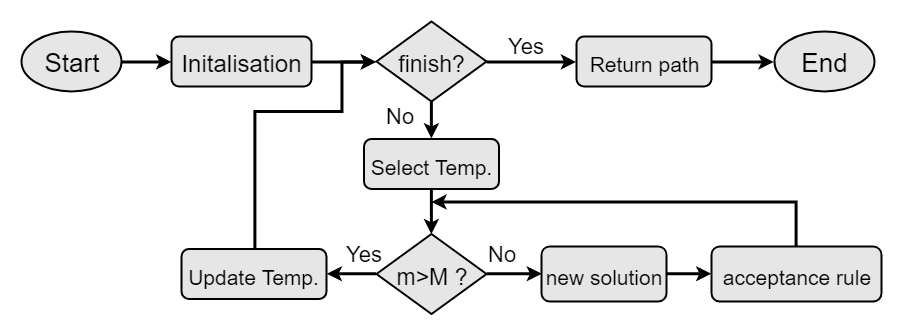
\includegraphics[width=\textwidth]{./Figures/system_implementation/LBSA.png}
  \caption{Block diagram of the Simmulated Annealing metaheuristic.}
  \label{fig:LBSA}  
\end{figure}

The majority of the SA algorithms operate on a single solution, but there are authors which 
propose a multi-agent approach \cite{multi_agent_SA}, and mention that the classic 
SA does not learn from its search history in an inteligent way, as other meta-heuristics, like the ACO, does.
Other authors focus on creating a cooling schedule which may benefit the SA algorithm, 
by enabling a more exhaustive exploration of the search space around more promosing temperatures.
An example of this is the List-Based SA algorithm proposed in \cite{list_based_SA},
which creates a cooling schedule which initially decreases faster than the traditional geometric schedule,
escaping faster from the non promising temperatures, and which than decreases slowly,
inducing a more exhaustive search around promising temperatures.  
The implementation of the Simmulated Annealing algorithm developed in this work,
follows the multi-agent and list-based chooling schedule, introduced in \cite{multi_agent_SA} and \cite{list_based_SA}.

Following the block diagram illustrated in fig \ref{fig:LBSA}, 
the algorithm receives a weight matrix describing the problem, and other relevant information,
as the duration associated to each city, and possible constraints relating the initial and final node.
The algorithm is than initialised, and some parameters must be set. This includes the initial acceptance probability $p_0$,
the maximum length of the temperature list $L_max$, the main cycle stop criteria and the markov cycle length.
The initialisation also requires the construction of an initial temperature list, which is done as follows: 

% TEMPERATURE LIST INITIALISATION
\begin{enumerate}[noitemsep,topsep=0pt,parsep=0pt,partopsep=0pt]
  \item Create an empty temperature list $L$;
  \item Create an initial solution $x$; 
  \item Create a candidate solution $y$ from $x$;
  \item If $f(y) < f(x)$, swap $x$ and $y$;
  \item Insert $t = \frac{-|f(y)-f(x)|}{p_0}$ into the temperature list;
  \item Repeat steps iii) to v) untill the temperature list reaches its maximum length;  
\end{enumerate}


The Simmulated Annealing metaheuristic is based on two cycles.
The inner cycle, often called the \textit{Markov chain},
is responsible for producing candidate solutions based on the current one.
The algorithm may accept or reject this candidate solution,
and this depends on the solutions objective function value, aswell as the current state temperature.
The Markov cycle usually runs for a fixed number of times, at each main iteration cycle.
After completing the Markov cycle, the temperature is decreased, 
and if the termination condition is not met, the Markov cycle restarts.

The process by which a candidate solution is generated is problem specific.
For the Traveling Salesman Problem, there are several suggestions in the literature,
which include, but are not limited to, 2 and 3-opt moves, insertion, reversion and swapping mechanisms.
During the development of this work, two stategies were tested.
The first follows a simple 2-opt move strategy at each markov cycle,
while the second is a greedy approach which selects the best result of the insertion, reversion and swapping functions.

At each step of the markov chain, the algorithm dictates 
that if a candidade solution is better than the current one, this solution is accepted,
and set as the current one. In its turn, if a candidate solution is worse,
it not automatically discarded, but it may be accepted.
This set of rules is refered to as the Metropolis acceptance criteria, and is defines in equation \ref{eq:metropolis_acceptance}.
The criteria sets that when confronted with a worse solution,
a random number $r: r \in [0, 1[$ is generated, and if $r$ is less than the acceptance probability, $e^{-\frac{f(y)-f(x)}{t}}$,
the candidate solution is accepted. 
This probability is such that, the lower the objective function difference,
the higher the probability of accepting the solution. On the contrary, as the state temperature decreases,
so does the acceptance probability.  

% METROPOLIS ACCEPTANCE RULE
\begin{equation}
\label{eq:metropolis_acceptance}
  p =  \left \{
  \begin{aligned}
    & 1, && \text{if}\ f(y) \leq f(x),\\
    & e^{-\frac{f(y)-f(x)}{t}},&& \text{otherwise}
  \end{aligned} \right. 
\end{equation}
  
The Simulated Annealing convergence theory suggests that this algorithm is capable of reaching the global minima, 
  









